\chapter{Module Loader}
\label{ch:ML}
\section{Linking and loading}
When the execution of a command \verb|M.P| is requested,
module \verb|M| containing procedure \verb|P| must be loaded, unless it
\begin{itemize}
  \item already loaded for its another command had earlier been executed, or
  \item had been imported by another one before.
\end{itemize}
Modules are available in the form of so-called \emph{object files}, generated by the compiler.
The term \emph{loading} refers to the transfer of module code from file into main memory,
from where processors fetch individual instructions.
It involves also a certain amount of transformation as required by
\begin{itemize}
  \item the object file format on the one hand, and
  \item the storage layout, on the other.
\end{itemize}
A system typically consists of many modules,
and hence loading modules also involves linking them together,
in particular linking with already loaded ones.  Before loading,
\begin{itemize}
  \item references to another module's objects are relative to the base address of this one;
  \item the linking or binding process converts them into absolute addresses.
\end{itemize}
This process may require a significant amount of address computations.
But they're simple enough and can be executed very swiftly,
if the data are organized in an appropriate way.  Nevertheless and surprisingly, in many OSes
it needs more time than compilation.  The remedy, which system designers offer,
is to separate linking from loading:
\begin{itemize}
  \item A set of compiled modules is 1st linked into a object file with absolute addresses.
  \item The loader then merely transfers it into main store.
\end{itemize}

We consider it an unfortunate solution.  Instead of trying to
cure it with aid of an additional processing stage and tool,
it is wiser to remove the malady at its core, namely to speed up linking itself.

Indeed, there is no separate linker.  In Oberon,
they are integrated and fast enough to avoid any desire for pre-linking.
Furthermore, the system extensibility crucially depends on the possibility
to link additional modules to already loaded ones by calls from any module.
This is called \emph{dynamic loading}, with prelinked object files which is impossible.
\begin{itemize}
  \item Newly loaded simply refer to already loaded, whereas
  \item prelinked files lead to multiple copies of same module.
\end{itemize}

Evidently, the essence of linking is the conversion of
\begin{itemize}
  \item relative addresses as generated by the compiler for all external references, into
  \item absolute ones as required during program execution.
\end{itemize}
To proceed, we must consider an additional complication.

Assume that a module \verb|M1| is to be compiled
which is a client of (that is, it imports) \verb|M0|.
The interface of \verb|M1| - in the form of a symbol file - does not specify the entry addresses
of its exported procedures, but merely specifies a unique number (\verb|pno|) for each one of them.
The reason are:
\begin{itemize}
  \item In this way the implementation of \verb|M0| may be modified,
    causing a change of entry addresses without affecting its interface specification.  And
  \item a crucial property of the scheme of separate modules compilation:
    Changes of the implementation of \verb|M0| must not necessitate
    the recompilation of clients (\verb|M1|).
\end{itemize}
The consequence is
\begin{itemize}
  \item the binding of entry addresses to \verb|pno|s must be performed by the linker.
    To make this possible,
  \item the object file must contain a list (table) of its entry addresses,
    one for each \verb|pno| used as index to the table.
\end{itemize}

Similarly, the object file must contain a table of imported modules, containing their names.
An external reference in the program code then appears in the form of a pair consisting of
\begin{itemize}
  \item a module number (\verb|mno|) - used as index to the import table (of modules), and
  \item a procedure number (\verb|pno|) - used as index to the entry table of this module.
\end{itemize}

Certain linkage information must not only be provided in each object file,
but also be present along with each loaded module's program code,
because a module to be loaded must be linkable with modules loaded at any earlier time
without reading their object files again.

\section{Module representation}
The primary requirement is
\begin{quote}
  a system must be represented in a form that allows to add new modules quickly.
\end{quote}
What is a sensible representation for this purpose?
The simplest solution that comes to mind is a list of module blocks containing sections for
\begin{itemize}
  \item the global data,
  \item the program code, and perhaps
  \item meta data for the linking process.
\end{itemize}
The list is rooted in a variable global to the loader module, here called \verb|Modules|.
\begin{figure}[h!]
  \centering
  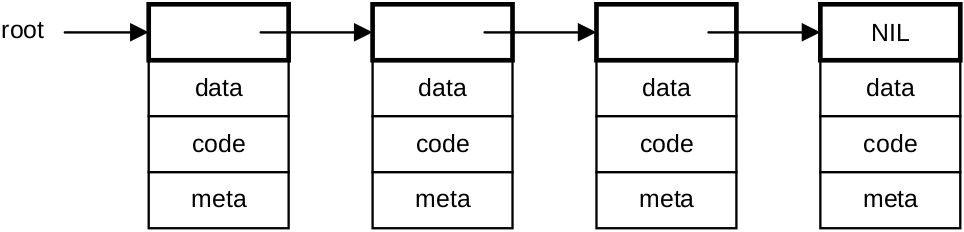
\includegraphics[width=\textwidth]{i/j}
  \caption{System of 4 modules}
  \label{fig:4modules}
\end{figure}

The 1st part, containing the link to the next module, is called \emph{module descriptor}.
In Oberon, it contains further links to the various sections of a module.
The type \verb|Module| is defined as:
\begin{verbatim}
  TYPE Module = POINTER TO ModDesc;
       ModuleName = ARRAY 32 OF CHAR;
       ModDesc = RECORD name: ModuleName;
                   next: Module;
                   key, num, size, refcnt, data, code,
                   imp, cmd, ent, ptr: INT (*addresses*)
                 END;
\end{verbatim}
\begin{itemize}
  \item[$key$] the module's key used for version consistency checking.
    Changes, if and only if, the module's interface and thereby its symbol file changes.
  \item[$num$] the module's number, index of the module's entry in a global module table,
    referenced by the processor's \verb|MT| register. The invariant relationship is \\
    \verb|    ModTable[mod.mno] = mod.data| \\ for all \verb|mod| in the module list.
  \item[$size$] the entire module block's size excluding the descriptor, and
  \item[$re\!f\!cnt$] the number of other modules importing this module.
    Used to check whether a module can be released by procedure \verb|Modules.Free|.
\end{itemize}
The section with meta data follows the \verb|data| and \verb|code| areas
and consists of several parts.
\begin{itemize}
  \item Imports is an array of the modules imported by this module,
    each entry being the address of the respective module descriptor.
  \item Commands is a sequence of procedure identifiers followed by their offset in the code section.
    This section is used when activating a command.
  \item Entries is an array of offsets of all exported entities (including commands).
    This section is used by the loader itself for linking.
  \item Pointer refs is an array of offsets of global pointer variables in the data section.
    These are used by the garbage collector as the roots of graphs of heap objects in use.
\end{itemize}
\begin{figure}[h!]
  \centering
  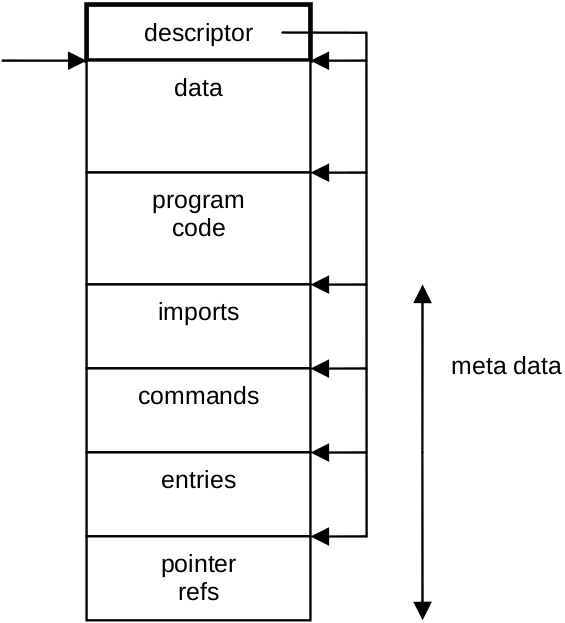
\includegraphics[width=.5\textwidth]{i/k}
  \caption{Module block headed by descriptor}
  \label{fig:module-block}
\end{figure}

\section{The linking loader}
The purpose of the loader is to read object files, and
to transform the file representation of modules into their internal image.

The loader is represented by procedure \verb|Load| in module \verb|Modules|.
It accepts a name and returns a pointer to the specified module's descriptor.
It 1st scans the list searching for the named module.
Only if it is not present, the module is loaded and added to the list.
Duplications therefore cannot occur.
\begin{verbatim}
  mod := root;
  WHILE (mod # NIL) & (name # mod.name) DO
    mod := mod.next
  END;

  IF mod = NIL THEN (*load*)
    F := ThisFile(name);
    Files.Set(R, F, 0);
    ...
\end{verbatim}

First, the header of the respective object file is read.
It specifies the required size of the block which is allocated in the module area
at the position indicated by the global variable \verb|AllocPtr|.
Then the list of imports of the module being imported is read,
and these module are imported.
Evidently procedure \verb|Load| is used recursively.
Because cyclic imports are excluded, recursion always terminates.
\begin{verbatim}
  Files.ReadString(R, impname); (*imports*)
  WHILE (impname[0] # 0X) & (res = 0) DO
    Files.ReadInt(R, impkey);
    Load(impname, impmod);
    import[nofimps] := impmod;
    importing := name1;
    IF res = 0 THEN
      IF impmod.key = impkey THEN
        INC(impmod.refcnt);
        INC(nofimps)
      ELSE
        error(3, name);
        imported := impname
      END
    END;
    Files.ReadString(R, impname)
  END
\end{verbatim}
The loading process stops, if a key mismatch is detected (\verb|err = 3|).
After successful loading of all imports,
the loading of the actual module proceeds by allocating a descriptor
and then reading the remaining sections of the file.
The data is allocated (and cleared) and the code section
is read in a straight-forward way without alteration.

At the very end of the file
3 integers called \verb|fixorgP|, \verb|fixorgD|, and \verb|fixorgT| are read.
They are the anchors of linked lists in the program code of instructions that need fixups.
These fixups are performed only after the entire file had been read.
Traversing the P-list, the pairs mno-pno are replaced by computed offsets
in \verb|BL| instructions (procedure calls).
Traversing the D-list, addresses of \verb|LDR| instructions and instruction pairs are fixed up,
and traversing the T-list, addresses of type descriptors are computed and inserted.
This low-level piece of code is shown below for call instructions (\verb|BL|).
Those for the D-List and the T-list are analogous.
\begin{verbatim}
  adr := mod.code + fixorgP*4;
  WHILE adr # mod.code DO
    SYSTEM.GET(adr, inst);
    mno := inst DIV 100000H MOD 10H; (*decompose*)
    pno := inst DIV 1000H MOD 100H;
    disp := inst MOD 1000H;
    SYSTEM.GET(mod.imp + (mno-1)*4, impmod);
    SYSTEM.GET(impmod.ent + pno*4, dest);
    dest := dest + impmod.code;
    offset := (dest - adr - 4) DIV 4;    (*compose*)
    SYSTEM.PUT(adr,(offset MOD 1000000H)+0F7000000H);
    adr := adr - disp*4
  END;
\end{verbatim}
After the module has been loaded successfully, its initialization body is executed.
Apart from \verb|Load|, module \verb|Modules| also contains the procedures
\begin{verbatim}
  PROC ThisCommand(mod: Module; name: ARRAY OF CHAR):
                                             Command;
  PROC Free       (             name: ARRAY OF CHAR);
\end{verbatim}
\begin{itemize}
  \item The former yields the procedure named \verb|name| from module \verb|mod|.
    It is used in \verb|TextFrames.Call| for activating command procedures.
  \item The latter unloads the named module, i.e. removes it from the list of loaded modules.
\end{itemize}

The frequent use of the low-level procedures \verb|SYSTEM.GET| and \verb|SYSTEM.PUT|
is easily justified in base modules such as the loader or device drivers.
After all, here data are transferred into untyped main storage.

\section{The toolbox of the loader}
User commands directed to the loader are contained in module \verb|System|.
The toolbox offers the following 3 commands:
\begin{verbatim}
  System.ShowModules
  System.ShowCommands modname
  System.Free {modname}
\end{verbatim}
\begin{itemize}
  \item The 1st command opens a viewer and provides a list of all loaded modules.
    The list indicates the block length and the number of clients importing a module
    (the reference count).
  \item \verb|ShowCommands| opens a viewer and lists the commands provided by the specified module.
    The commands are prefixed by the module name,
    and hence can immediately be activated by a mouse click.
  \item \verb|Free| is called in order to remove modules either to regain storage space or
    to replace a module by a newly compiled version.
    A module can be dispensed only if
    \begin{enumerate}
      \item it has no clients, and
      \item does not declare any record types which are extensions of imported types.
    \end{enumerate}
\end{itemize}

\section{The Oberon object file format}
The name extension of object files is \verb|.rsc|.  Their syntax:
\begin{verbatim}
  CodeFile = name key version size
  imports typedesc varsize strings code commands
          entries ptrrefs fixP fixD fixT body "O".
  imports = {modname key} 0X.
  typedesc = nof {byte}.
  strings = nof {char}.
  code = nof {word}.
  commands = {comname offset} 0X.
  entries = nof {word}.
  ptrrefs = {word} 0.
\end{verbatim}
\begin{itemize}
  \item \verb|fixP|, \verb|fixD|, \verb|fixT| are the origins of chains of instructions to be updated (fixed up).
  \item \verb|body| is the entry point offset of the module \verb|body|.
\end{itemize}
